\subsection{FCOS-3D}
FCOS-3D is a single-stage network that extends FCOS~\cite{tian2019fcos} to perform 3D detection and dense depth prediction. It is composed of backbone network and three \emph{subnetworks}. As in \cite{tian2019fcos}, we adopt feature pyramid network(FPN)~\cite{} 
\begin{figure}[h]
	\centering
	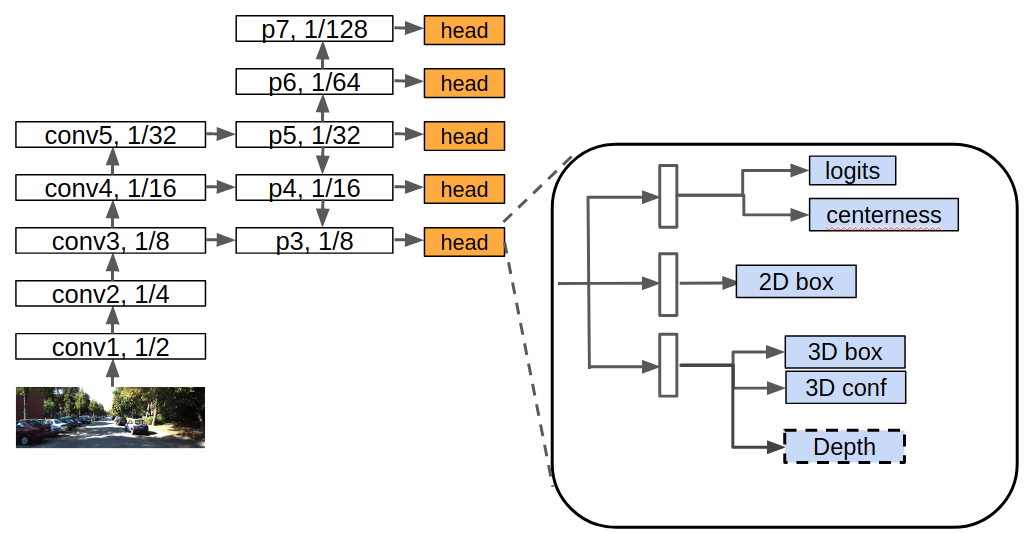
\includegraphics[width=1.0\columnwidth]{figures/fcos3d_arch.png}
	\caption{FCOS-3D extends FCOS to perform 3D detection and dense depth prediction. As in FCOS, a shared head is applied to all levels of FPN features, but with one exception: the depth head is only applied on to the highest resolution features (i.e. $\texttt{p3}$ features).}
\end{figure}

\begin{itemize}
    \item FCOS3D extends FCOS to predict 3D bounding box, in addition to category labels and 2D bounding box.
    \item The output of 3D box head consists of projected centroid, depth of centroid, and size of the 3D box.
    \item Backbone: DLA-34
    \item Matching: Given a 2D bounding box of a foreground object, we associate the features that are within $R$ pixels from the center of 2D bounding box with the given instance.
    \item Loss function: We use disentangled 3D box loss introduced in MonoDis.
    \item 3D confidence: As in MonoDis, we use the 3D confidence, predicted by an additional head, to reweight the logit-based classification score
\end{itemize}

\subsection{Depth pretraining for FCOS-3D}
Dataset: IODA dataset consist of 3.4M pairs or image and Lidar pointcloud. The dataset covers diverse urban environment across US and Japan. The pointcloud is captured by high-resolution Luminar device.
\begin{itemize}
    \item We extend FCOS-3D to perform dense prediction task by aggregating the output of conv2D layer of 3D box head. That is, we upsample all low-resolution features, and add them to produce a dense (stride=4) feature map, and compute depth estimation.
    \item Loss function: we investigate various loss functions, and conclude L1-loss works best. 
    \item Range-aware pretraining. The most challenging instances in monocular 3D detection are in 20-40m range. Therefore, we investigate whether focusing on this range of depth in pretraining helps.
    \item Scale law: We investigate how much of image-pointcloud pairs are needed for a good transfer.
\end{itemize}
\subsection{Depth fine-tuning for FCOS-3D}
\begin{itemize}
    \item Once pretrained, we fine-tune FCOS-3D in multi-task framework, using KITTI3D dataset.
    \item We project Lidar points onto image plane, and use the same archiecture for pretraining to predict sparse per-pixel depth, in addition to the original FCOS-3D losses.
\end{itemize}